\section{Исследовательская часть}

\subsection{Технические характеристики}

Технические характеристики устройства, на котором выполнялся замерный эксперимент:
\begin{itemize}[label*=---]
	\item операционная система Windows 11;
	\item память 16 ГБ;
	\item процессор 3,6 ГГц 6-ядерный процессор AMD Ryzen 5000 series 5.
\end{itemize}

Замеры проводилось на ноутбуке, включенном в сеть электропитания. 
Во время тестирования ноутбук был нагружен только интегрированной средой разработки и непосредственно выполняемой программой.

\subsection{Пример работы программы}

На рисунке \ref{img:example} представлен пример работы программы. 
Вводятся две строки. 
Для этих строк высчитывается расстояние Левенштейна и Дамерау-Левенштейна.
Выводится результат вычислений и время работы каждого алгоритма в микросекундах. 

\begin{figure}[!h]
	\centering
	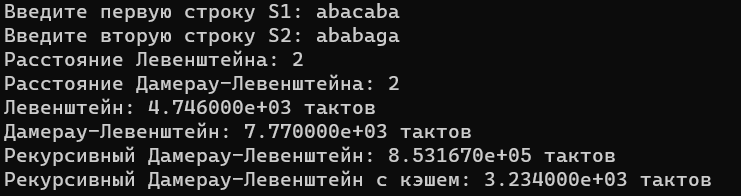
\includegraphics[width=130mm]{images/example}
	\caption{Пример работы программы}
	\label{img:example}
\end{figure}

\pagebreak
\newpage
\subsection{Время выполнения реализованных алгоритмов}

Введём следующие обозначения:
\begin{description}
	\item[Л] - Левенштейна
	\item[ДЛ] - Дамерау~---~Левенштейн
	\item[РДЛ] - Рекурсивный Дамерау~---~Левенштейн
	\item[РДЛК] - Рекурсивный Дамерау~---~Левенштейн с кэшем
\end{description}

\begin{table}[hbtp]
	\centering
	\caption{Результаты замеров времени реализованных алгоритмов в тактах процессора}
	\label{tab:time}
	\csvreader[
	tabular=|r|r|r|r|r|,
	table head=\hline Длина строк & Л & ДЛ & РДЛ & РДЛК \\ \hline,
	late after last line=\\\hline,
	]{time.csv}{}{\csvlinetotablerow}
\end{table}

Замеры времени работы реализованных алгоритмов для определенной длины строк проводились 100 раз, при этом каждый раз строки генерировались случайно.
Для измерения тактового времени была использована инструкция rdtsc \cite{microsoft_rdtsc}.
В качестве результата, представленного в таблице \ref{tab:time}, взято среднее время на каждой длине слова.

\pagebreak
\newpage

\subsection{Занимаемая память реализованных алгоритмов}

В данном разделе представлены результаты замеров затрат памяти для различных алгоритмов на обработку строк разной длины. 
Таблица \ref{tab:memory} демонстрирует объем памяти в байтах, потребляемый разными реализациями алгоритмов в зависимости от длины обрабатываемых строк.

\begin{table}[ht]
	\centering
	\caption{Затраты памяти в байтах для различных алгоритмов в зависимости от длины строк}
	\label{tab:memory}
	\csvreader[
	tabular=|r|r|r|r|r|,
	table head=\hline N & Л & ДЛ & РДЛ & РДЛК \\ \hline,
	late after last line=\\\hline,
	]{memory.csv}{}{\csvlinetotablerow}
\end{table}

\subsection{Вывод}

В результате анализа замеров времени выполнения и затрат памяти на различных алгоритмах были сделаны следующие выводы:

\begin{itemize}
	\item для обработки строк длины меньшей, чем пять символов, рекомендуется использовать рекурсивные алгоритмы;
	\item для строк, содержащих больше пяти символов, рекомендуется использовать итеративные алгоритмы, т.к. они предоставляют лучшую производительность;
	\item при необходимости учета транспозиций символов алгоритм Дамерау~---~Левенштейна с кэшированием (РДЛК) является предпочтительным выбором.
\end{itemize}